\documentclass[14pt]{extbook}
\usepackage{multicol, enumerate, enumitem, hyperref, color, soul, setspace, parskip, fancyhdr} %General Packages
\usepackage{amssymb, amsthm, amsmath, latexsym, units, mathtools} %Math Packages
\everymath{\displaystyle} %All math in Display Style
% Packages with additional options
\usepackage[headsep=0.5cm,headheight=12pt, left=1 in,right= 1 in,top= 1 in,bottom= 1 in]{geometry}
\usepackage[usenames,dvipsnames]{xcolor}
\usepackage{dashrule}  % Package to use the command below to create lines between items
\newcommand{\litem}[1]{\item#1\hspace*{-1cm}\rule{\textwidth}{0.4pt}}
\pagestyle{fancy}
\lhead{Progress Quiz 5}
\chead{}
\rhead{Version C}
\lfoot{8497-6012}
\cfoot{}
\rfoot{Summer C 2021}
\begin{document}

\begin{enumerate}
\litem{
Construct the lowest-degree polynomial given the zeros below. Then, choose the intervals that contain the coefficients of the polynomial in the form $x^3+bx^2+cx+d$.\[ 4 - 2 i \text{ and } -4 \]\begin{enumerate}[label=\Alph*.]
\item \( b \in [2.8, 5.1], c \in [-12, -11], \text{ and } d \in [-87, -78] \)
\item \( b \in [-7.8, -3.5], c \in [-12, -11], \text{ and } d \in [78, 84] \)
\item \( b \in [-0.6, 1.1], c \in [3, 7], \text{ and } d \in [3, 9] \)
\item \( b \in [-0.6, 1.1], c \in [0, 5], \text{ and } d \in [-20, -13] \)
\item \( \text{None of the above.} \)

\end{enumerate} }
\litem{
Construct the lowest-degree polynomial given the zeros below. Then, choose the intervals that contain the coefficients of the polynomial in the form $ax^3+bx^2+cx+d$.\[ -6, \frac{1}{3}, \text{ and } \frac{-3}{2} \]\begin{enumerate}[label=\Alph*.]
\item \( a \in [6, 12], b \in [-25.3, -24.5], c \in [-64, -61], \text{ and } d \in [-24, -15] \)
\item \( a \in [6, 12], b \in [40.1, 45.7], c \in [33, 40], \text{ and } d \in [-24, -15] \)
\item \( a \in [6, 12], b \in [-30.7, -26], c \in [-53, -38], \text{ and } d \in [11, 26] \)
\item \( a \in [6, 12], b \in [-44.1, -41], c \in [33, 40], \text{ and } d \in [11, 26] \)
\item \( a \in [6, 12], b \in [40.1, 45.7], c \in [33, 40], \text{ and } d \in [11, 26] \)

\end{enumerate} }
\litem{
Describe the end behavior of the polynomial below.\[ f(x) = -6(x + 7)^{5}(x - 7)^{10}(x - 8)^{3}(x + 8)^{3} \]\begin{enumerate}[label=\Alph*.]
\begin{multicols}{2}\item 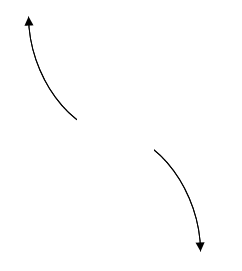
\includegraphics[width = 0.3\textwidth]{../Figures/polyEndBehaviorAC.png}\item 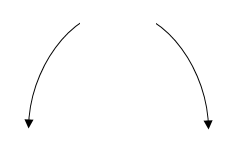
\includegraphics[width = 0.3\textwidth]{../Figures/polyEndBehaviorBC.png}\item 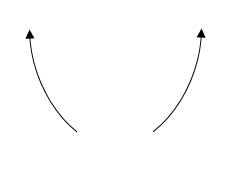
\includegraphics[width = 0.3\textwidth]{../Figures/polyEndBehaviorCC.png}\item 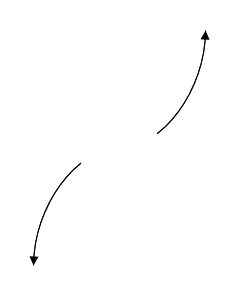
\includegraphics[width = 0.3\textwidth]{../Figures/polyEndBehaviorDC.png}\end{multicols}\item None of the above.
\end{enumerate} }
\litem{
Which of the following equations \textit{could} be of the graph presented below?
\begin{center}
    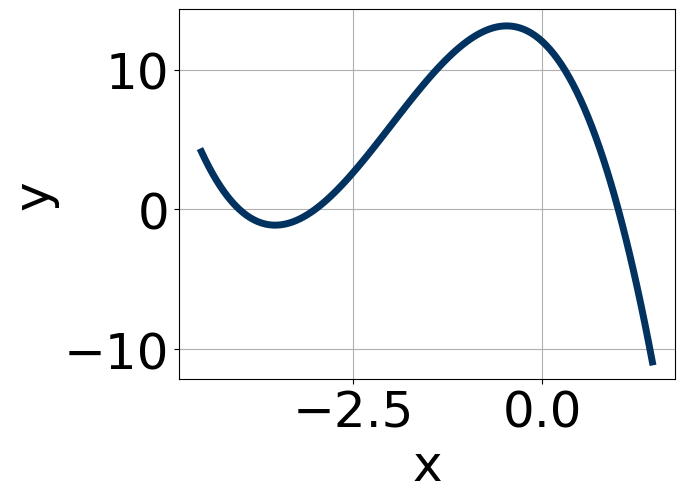
\includegraphics[width=0.5\textwidth]{../Figures/polyGraphToFunctionCopyC.png}
\end{center}
\begin{enumerate}[label=\Alph*.]
\item \( -10(x + 3)^{10} (x - 1)^{11} (x + 4)^{9} \)
\item \( 9(x + 3)^{10} (x - 1)^{5} (x + 4)^{5} \)
\item \( 16(x + 3)^{7} (x - 1)^{7} (x + 4)^{5} \)
\item \( -17(x + 3)^{10} (x - 1)^{6} (x + 4)^{11} \)
\item \( -13(x + 3)^{9} (x - 1)^{7} (x + 4)^{5} \)

\end{enumerate} }
\litem{
Construct the lowest-degree polynomial given the zeros below. Then, choose the intervals that contain the coefficients of the polynomial in the form $ax^3+bx^2+cx+d$.\[ \frac{1}{4}, \frac{7}{4}, \text{ and } \frac{-2}{3} \]\begin{enumerate}[label=\Alph*.]
\item \( a \in [45, 50], b \in [123, 130], c \in [83, 89], \text{ and } d \in [12, 19] \)
\item \( a \in [45, 50], b \in [-41, -33], c \in [-70, -66], \text{ and } d \in [-20, -13] \)
\item \( a \in [45, 50], b \in [-66, -60], c \in [-43, -33], \text{ and } d \in [12, 19] \)
\item \( a \in [45, 50], b \in [-66, -60], c \in [-43, -33], \text{ and } d \in [-20, -13] \)
\item \( a \in [45, 50], b \in [64, 70], c \in [-43, -33], \text{ and } d \in [-20, -13] \)

\end{enumerate} }
\litem{
Which of the following equations \textit{could} be of the graph presented below?
\begin{center}
    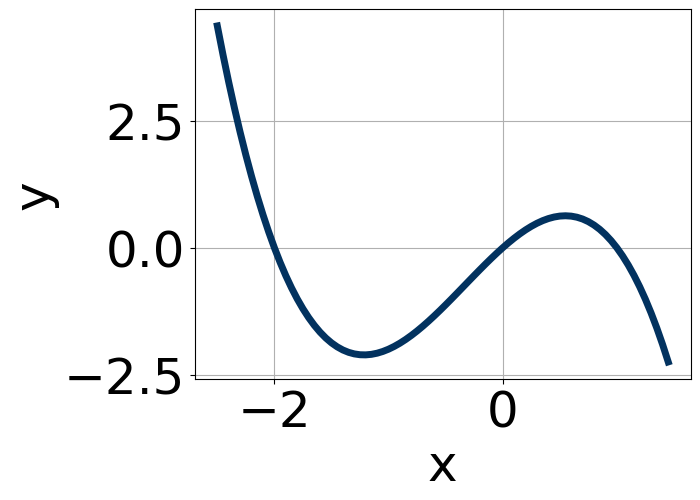
\includegraphics[width=0.5\textwidth]{../Figures/polyGraphToFunctionC.png}
\end{center}
\begin{enumerate}[label=\Alph*.]
\item \( 11x^{9} (x + 2)^{6} (x - 1)^{5} \)
\item \( 11x^{11} (x + 2)^{5} (x - 1)^{5} \)
\item \( -12x^{5} (x + 2)^{5} (x - 1)^{9} \)
\item \( -6x^{7} (x + 2)^{10} (x - 1)^{7} \)
\item \( -9x^{6} (x + 2)^{4} (x - 1)^{7} \)

\end{enumerate} }
\litem{
Describe the zero behavior of the zero $x = -8$ of the polynomial below.\[ f(x) = 3(x + 2)^{5}(x - 2)^{2}(x + 8)^{7}(x - 8)^{2} \]\begin{enumerate}[label=\Alph*.]
\begin{multicols}{2}\item 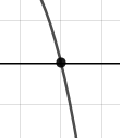
\includegraphics[width = 0.3\textwidth]{../Figures/polyZeroBehaviorAC.png}\item 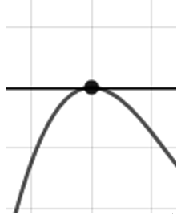
\includegraphics[width = 0.3\textwidth]{../Figures/polyZeroBehaviorBC.png}\item 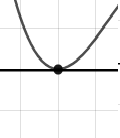
\includegraphics[width = 0.3\textwidth]{../Figures/polyZeroBehaviorCC.png}\item 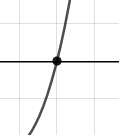
\includegraphics[width = 0.3\textwidth]{../Figures/polyZeroBehaviorDC.png}\end{multicols}\item None of the above.
\end{enumerate} }
\litem{
Describe the zero behavior of the zero $x = -5$ of the polynomial below.\[ f(x) = 7(x - 5)^{2}(x + 5)^{5}(x + 9)^{8}(x - 9)^{11} \]\begin{enumerate}[label=\Alph*.]
\begin{multicols}{2}\item 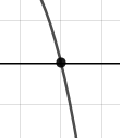
\includegraphics[width = 0.3\textwidth]{../Figures/polyZeroBehaviorCopyAC.png}\item 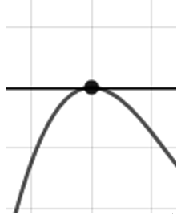
\includegraphics[width = 0.3\textwidth]{../Figures/polyZeroBehaviorCopyBC.png}\item 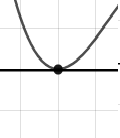
\includegraphics[width = 0.3\textwidth]{../Figures/polyZeroBehaviorCopyCC.png}\item 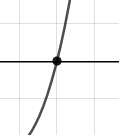
\includegraphics[width = 0.3\textwidth]{../Figures/polyZeroBehaviorCopyDC.png}\end{multicols}\item None of the above.
\end{enumerate} }
\litem{
Construct the lowest-degree polynomial given the zeros below. Then, choose the intervals that contain the coefficients of the polynomial in the form $x^3+bx^2+cx+d$.\[ -4 + 3 i \text{ and } 3 \]\begin{enumerate}[label=\Alph*.]
\item \( b \in [-0.5, 2], c \in [-15, -4], \text{ and } d \in [7, 12] \)
\item \( b \in [3.6, 8.1], c \in [0, 5], \text{ and } d \in [-77, -74] \)
\item \( b \in [-5.2, 0.5], c \in [0, 5], \text{ and } d \in [70, 77] \)
\item \( b \in [-0.5, 2], c \in [0, 5], \text{ and } d \in [-14, -5] \)
\item \( \text{None of the above.} \)

\end{enumerate} }
\litem{
Describe the end behavior of the polynomial below.\[ f(x) = 5(x - 6)^{2}(x + 6)^{3}(x + 3)^{5}(x - 3)^{7} \]\begin{enumerate}[label=\Alph*.]
\begin{multicols}{2}\item 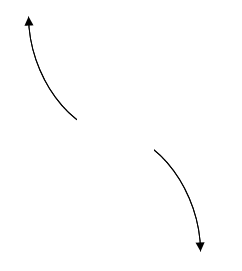
\includegraphics[width = 0.3\textwidth]{../Figures/polyEndBehaviorCopyAC.png}\item 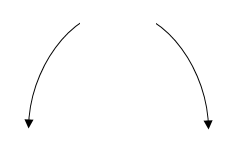
\includegraphics[width = 0.3\textwidth]{../Figures/polyEndBehaviorCopyBC.png}\item 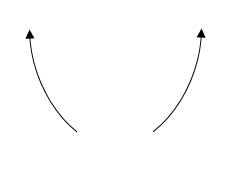
\includegraphics[width = 0.3\textwidth]{../Figures/polyEndBehaviorCopyCC.png}\item 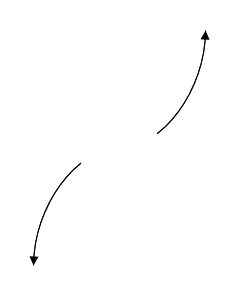
\includegraphics[width = 0.3\textwidth]{../Figures/polyEndBehaviorCopyDC.png}\end{multicols}\item None of the above.
\end{enumerate} }
\end{enumerate}

\end{document}